\documentclass{beamer}
\usepackage[english, russian]{babel}
\usepackage[T2A]{fontenc}
\usepackage[utf8]{inputenc}
\usepackage{indentfirst}
\usepackage{amsmath, amsfonts, amssymb, amsthm, mathtools}
\usepackage[export]{adjustbox}
\usepackage{graphicx} 
\graphicspath{ {./images/} }

\usepackage{subcaption}
\usepackage{verbatim}

\usepackage{minted}{\setlength{\parskip}{0pt}}

\usepackage{hyperref}

\hypersetup{
    colorlinks=true,
    linkcolor=blue,
    filecolor=magenta,      
    urlcolor=black,
    pdftitle={Overleaf Example},
    pdfpagemode=FullScreen,
    }


\title{Отчет по лабораторной работе № 1. \\ Подготовка лабораторного стенда.}
\author{Данила Стариков \\ НПИбд-02-22}
\date{2024}

\begin{document}

\maketitle
\newpage

\tableofcontents

\newpage
\section{Цель работы}

Целью данной работы является приобретение практических навыков установки Rocky Linux на виртуальную машину с помощью инструмента Vagrant.

\newpage
\section{Выполнение работы}
\subsection{Подготовка рабочего каталога}

Подготовка лабораторного стенда проводилась в ОС Linux. Предварительно были установлены:
\begin{itemize}
    \item Vagrant v2.3.4 (\url{https://vagrantup.com});
    \item VirtualBox v7.0.16 (\url{https://www.virtualbox.org}). Стоит отметить, что по умолчанию пакетный менеджер \texttt{dnf} устанавливает версию 7.1.0, в которой присутствует ошибка с настройкой опции графического ускорения, что не позволяет собрать \texttt{box}\-файл. Откат к прошлой версии устарняет проблему.
    \item Packer v1.11.2 (\url{https://www.packer.io}).
\end{itemize}

Перед началом работы создан временный каталог \texttt{~/tmp/dastarikov}, в котором проводилась работа. В нем расположили образ ОС Rocky Linux v9.4  (\url{https://www.rockylinux.org/download}), и 2 подкаталога \texttt{packer} и \texttt{vagrant}, где находятся скрипты и конфигурационные файлы, необходимые для сборки \texttt{box}\-файла (Рис. \ref{img:1}).
\begin{center}
    \centering
    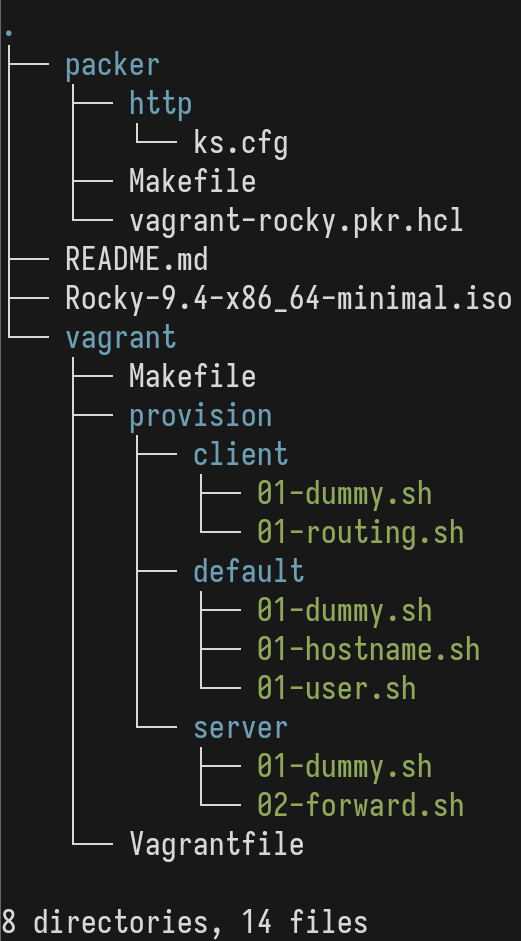
\includegraphics[width=0.5\textwidth]{../images/img1.png}
    \captionof{figure}{Структура рабочего каталога.}
    \label{img:1}
\end{center}

Сделали несколько изменений в файлах конфигурации: в файлах \texttt{vagrant/default/01-user.sh} и \texttt{vagrant/default/01-hostname.sh} присвоили переменной \texttt{username} значение \texttt{dastarikov}.

\subsection{Рарзвертывание лабораторного стенда на ОС Linux}

\begin{enumerate}
    \item Перешли в каталог с проектом (в нем также должен располагаться образ OC Rocky Linux):
        \begin{minted}{bash}
        cd /var/tmp/dastarikov/packer
        \end{minted}
    \item В терминале набрали
        \begin{minted}{bash}
        makе help
        \end{minted}
    \item Для формирования \texttt{box}\-файла с дистрибутивом Rocky Linux для VirtualBox в терминале набрали (Рис. \ref{img:2})
        \begin{minted}{bash}
        make init
        make box
        \end{minted}
    \begin{center}
        \centering
        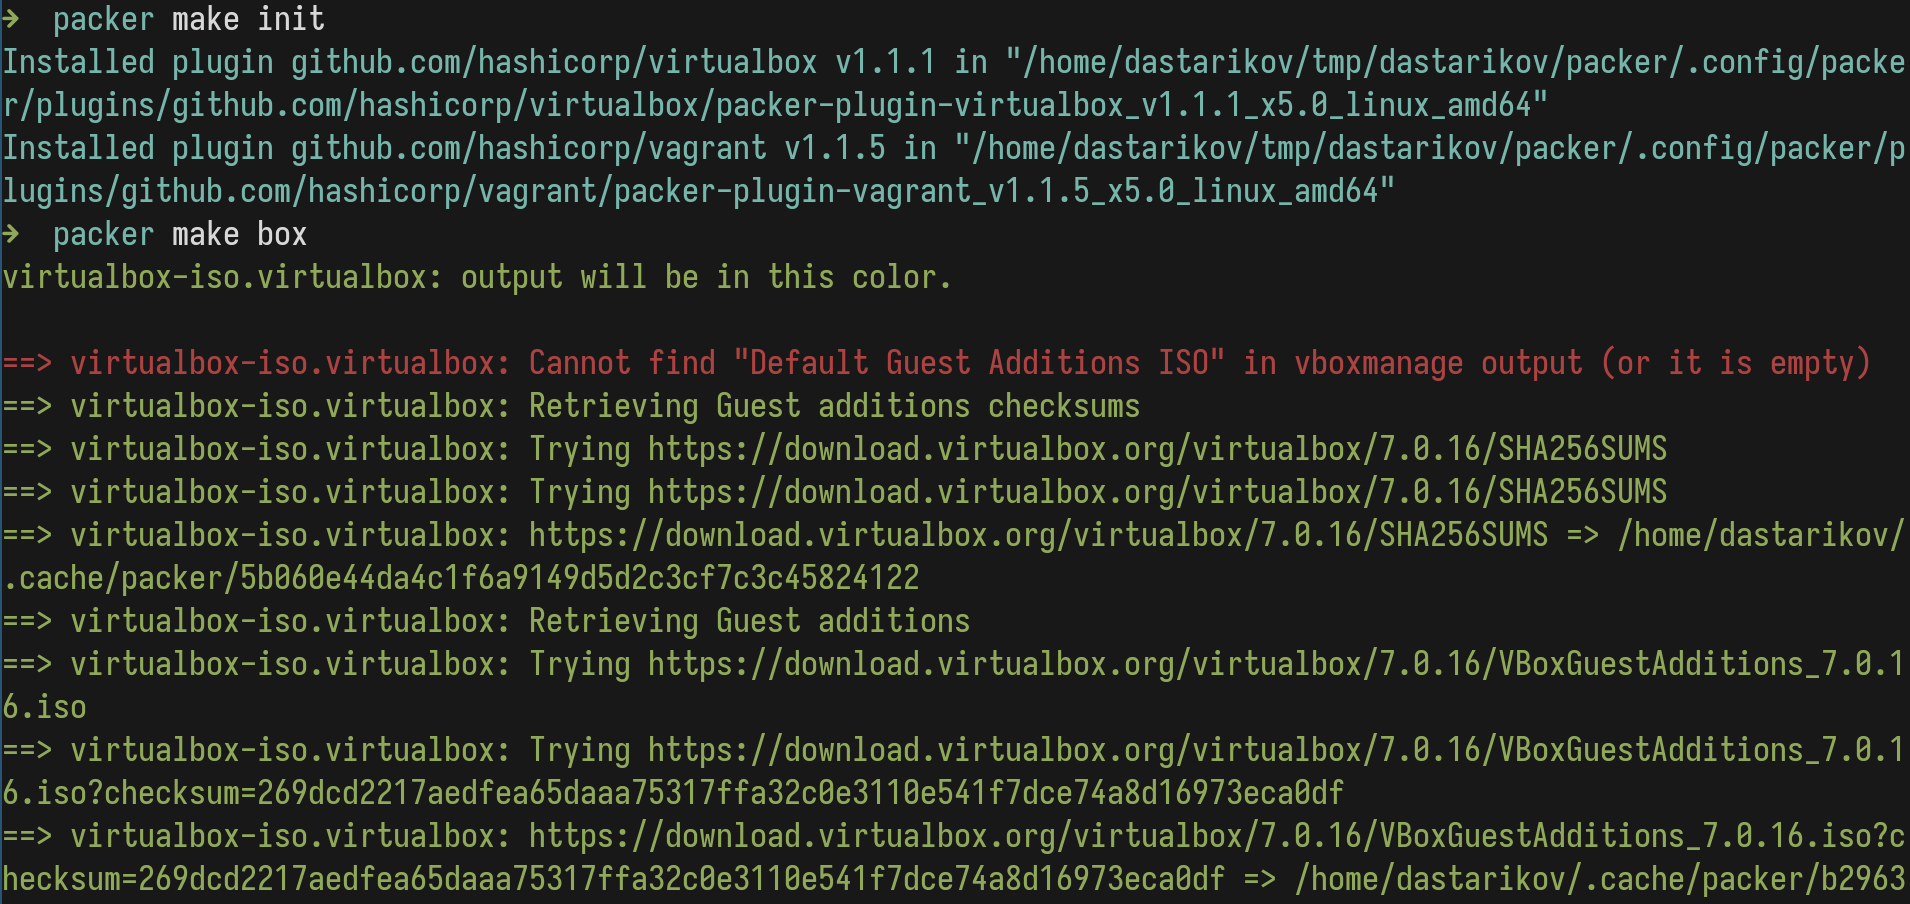
\includegraphics[width=0.7\textwidth]{../images/img2.png}
        \captionof{figure}{Запуск формирования \texttt{box}\-файла.}
        \label{img:2}
    \end{center}

    \item Далее начнинается процесс скачивания, распаковки и установки драйверов VirtualBox и дистрибутива на виртуальную машину. После завершения в каталоге \texttt{packer} сформировался образ \texttt{vagrant-virtualbox-rocky-9-x86\_64.box} (Рис. \ref{img:3}).
    \begin{center}
        \centering
        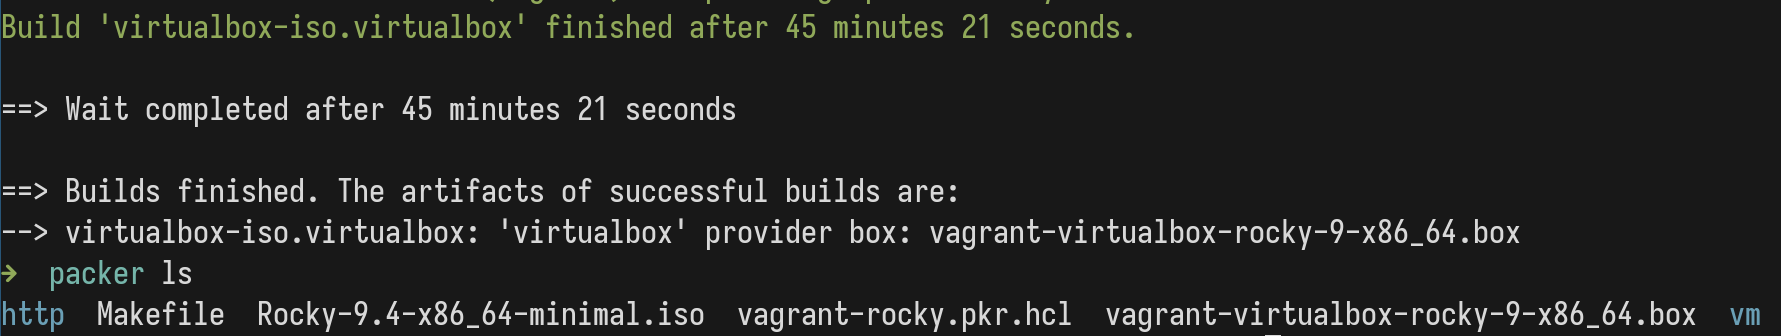
\includegraphics[width=0.7\textwidth]{../images/img3.png}
        \captionof{figure}{Окончание сброки образа.}
        \label{img:3}
    \end{center}

    \item Скопировали файл \texttt{vagrant-virtualbox-rocky-9-x86\_64.box} в рабочий каталог в подкаталог \texttt{vagrant}.
    \item Для регистрации образа виртуальной машины в Vagrant в терминале в каталоге \texttt{vagrant} набрали (Рис. \ref{img:4})
        \begin{minted}{bash}
        make addbox
        \end{minted}
    \item Запустили виртуальную машину Server (Рис. \ref{img:5}), введя
        \begin{minted}{bash}
        make server-up
        \end{minted}
    \item Запустили виртуальную машину Client (Рис. \ref{img:6}), введя
        \begin{minted}{bash}
        make client-up
        \end{minted}
    \begin{center}
        \centering
        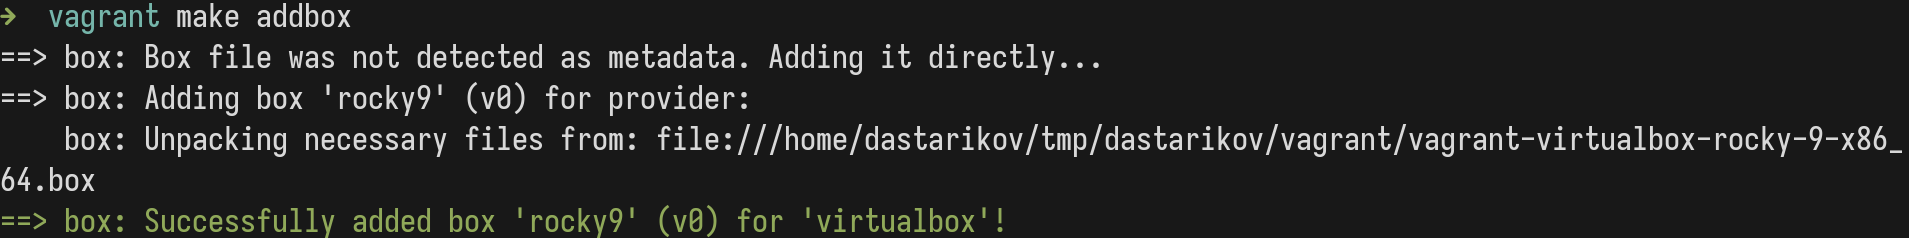
\includegraphics[width=0.7\textwidth]{../images/img4.png}
        \captionof{figure}{Регистрация образа в Vagrant.}
        \label{img:4}
    \end{center}
    \begin{center}
        \centering
        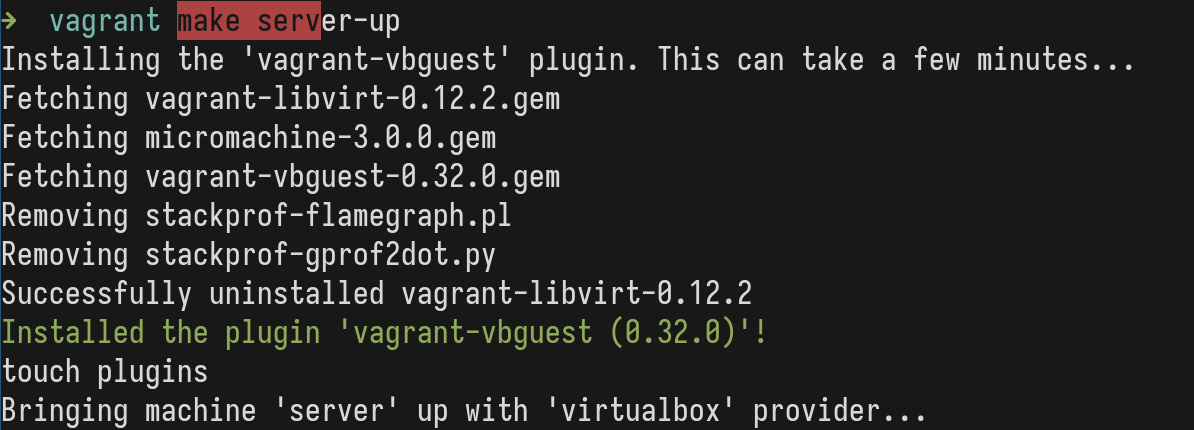
\includegraphics[width=0.7\textwidth]{../images/img5.png}
        \captionof{figure}{Запуска виртуальной машины server}
        \label{img:5}
    \end{center}
    \begin{center}
        \centering
        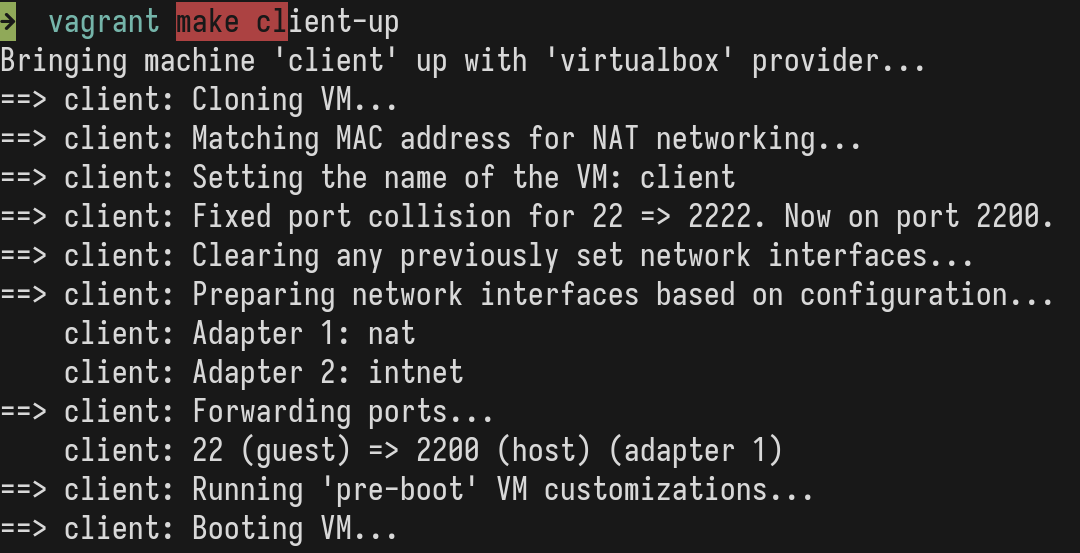
\includegraphics[width=0.7\textwidth]{../images/img6.png}
        \captionof{figure}{Запуска виртуальной машины client}
        \label{img:6}
    \end{center}
    \item Подключились к серверу из консоли (Рис. \ref{img:7}):
        \begin{minted}{bash}
        vagrant ssh server
        \end{minted}
    \item Ввели пароль \texttt{vagrant}.
    \item Перешли к пользователю dastarikov
        \begin{minted}{bash}
        su - dastarikov
        \end{minted}
    \item Отлогинились.
    \item Проделали тоже самое для клиента (Рис. \ref{img:7a}).
    \begin{center}
        \centering
        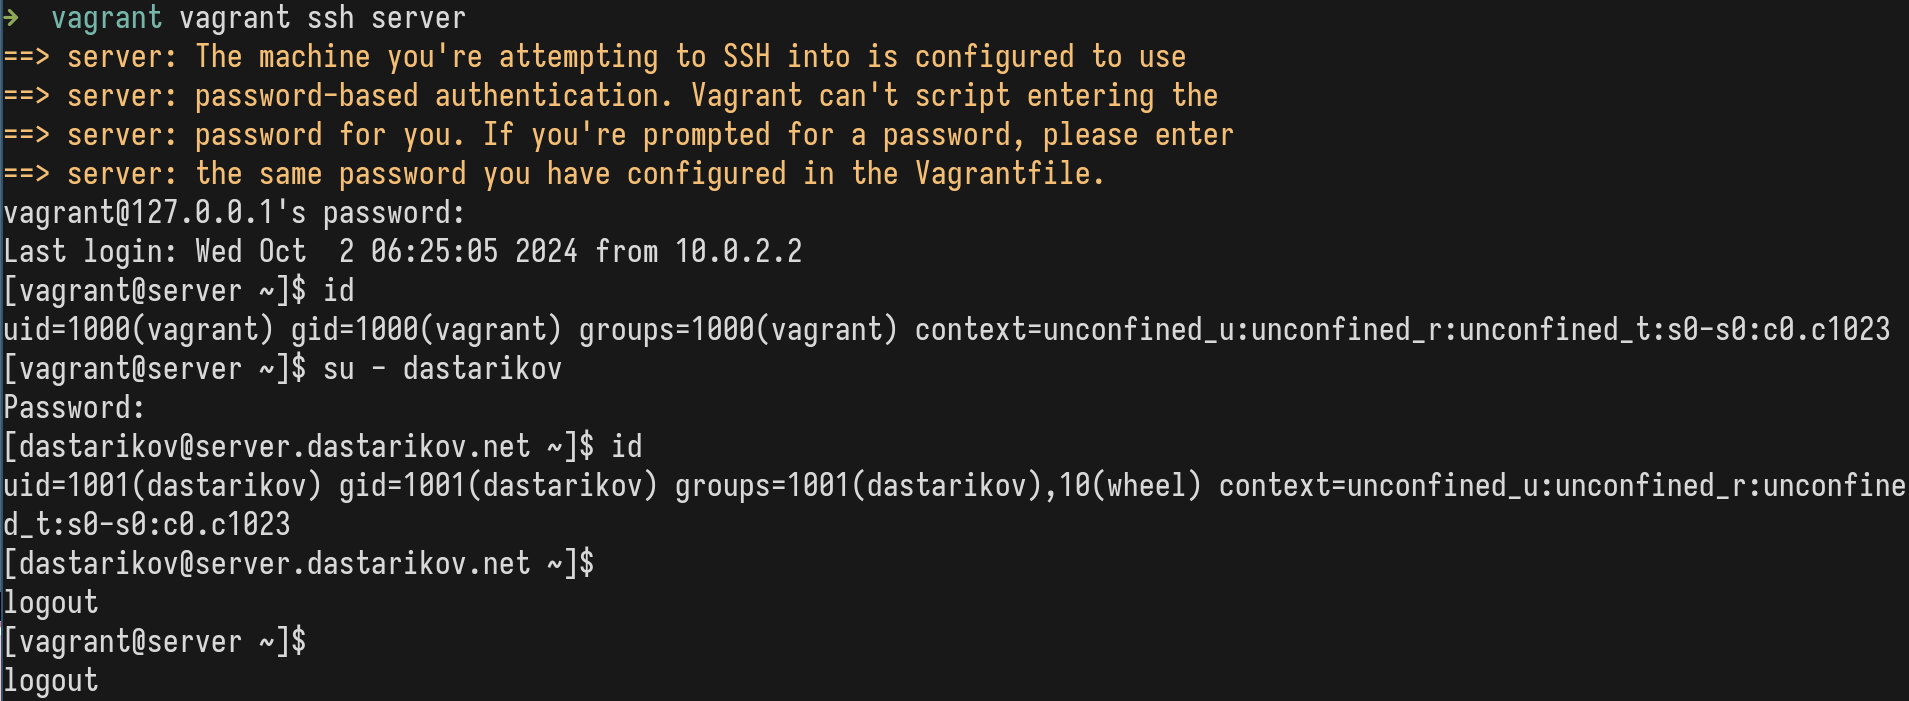
\includegraphics[width=0.7\textwidth]{../images/img7.png}
        \captionof{figure}{Подключение к серверу из консоли.}
        \label{img:7}
    \end{center}
    \begin{center}
        \centering
        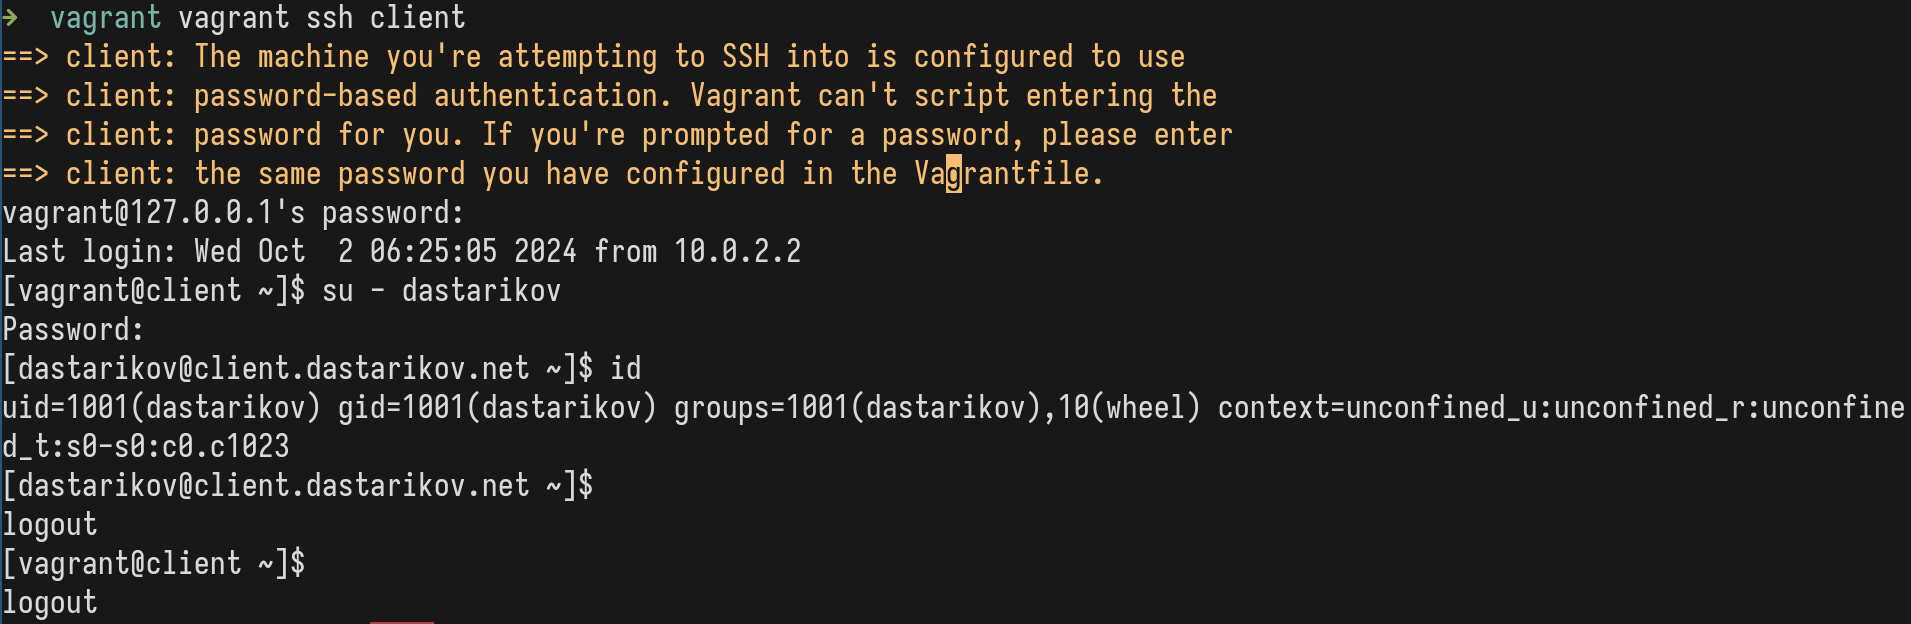
\includegraphics[width=0.7\textwidth]{../images/img7a.png}
        \captionof{figure}{Подключение к клиенту из консоли.}
        \label{img:7a}
    \end{center}
    \item Выключили обе виртуальные машины (Рис. \ref{img:8}):
        \begin{minted}{bash}
        make server-halt
        make client-halt
        \end{minted}
    \begin{center}
        \centering
        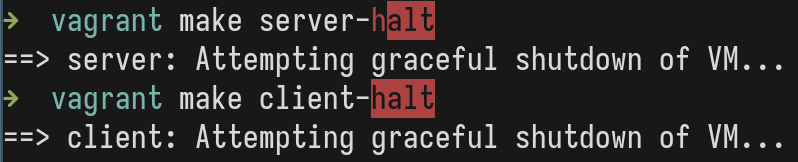
\includegraphics[width=0.7\textwidth]{../images/img8.png}
        \captionof{figure}{Выключение виртуальных машин.}
        \label{img:8}
    \end{center}
    \item Убедились, что запуск обеих виртуальных машин прошёл успешно, залогинились под пользователем \texttt{vagrant} с паролем \texttt{vagrant} в графическом окружении (Рис. \ref{img:9} и \ref{img:10}).
    \begin{center}
        \centering
        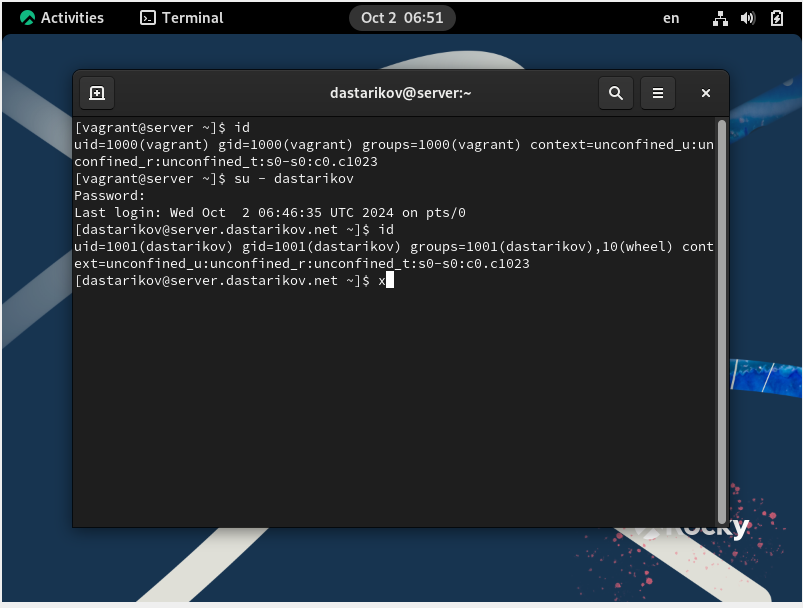
\includegraphics[width=0.7\textwidth]{../images/img9.png}
        \captionof{figure}{Работа в графическом окружении сервера.}
        \label{img:9}
    \end{center}
    \begin{center}
        \centering
        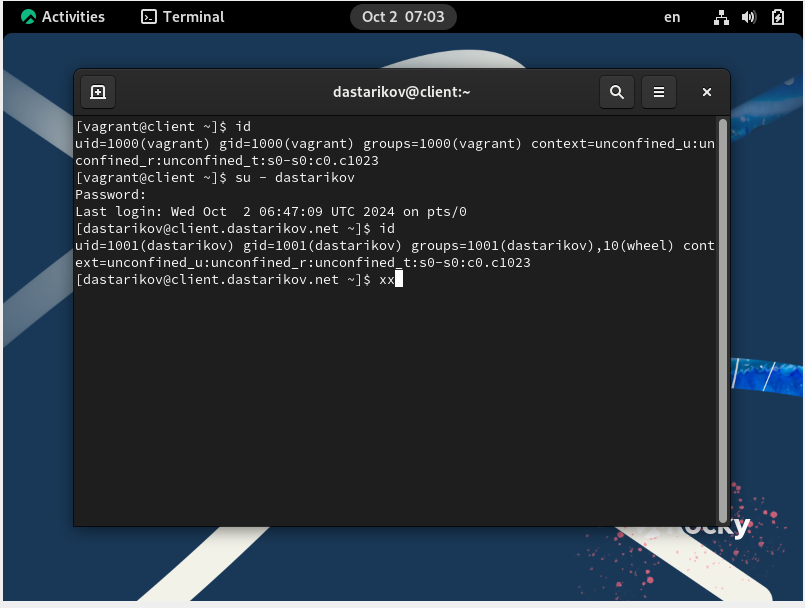
\includegraphics[width=0.7\textwidth]{../images/img10.png}
        \captionof{figure}{Работа в графическом окружении клиента.}
        \label{img:10}
    \end{center}
\end{enumerate}

\subsection{Внесение изменений в настройки внутреннего окружения виртуальной машины}

\begin{enumerate}
    \item Для отработки созданных скриптов во время загрузки виртуальных машин убедились, что в конфигурационном файле Vagrantfile до строк с конфигурацией сервера имеется следующая запись:
        \begin{minted}{bash}
        # Common configuration
        config.vm.provision "common user",
        type: "shell",
        preserve_order: true,
        path: "provision/default/01-user.sh"
        config.vm.provision "common hostname",
        type: "shell",
        preserve_order: true,
        run: "always",
        path: "provision/default/01-hostname.sh"
        \end{minted}
    \item Зафиксировали внесённые изменения для внутренних настроек виртуальных машин (Рис. \ref{img:11} и \ref{img:12}), введя в терминале:
        \begin{minted}{bash}
        make server-provision
        \end{minted}
    Затем
        \begin{minted}{bash}
        make client-provision
        \end{minted}
            \begin{center}
        \centering
        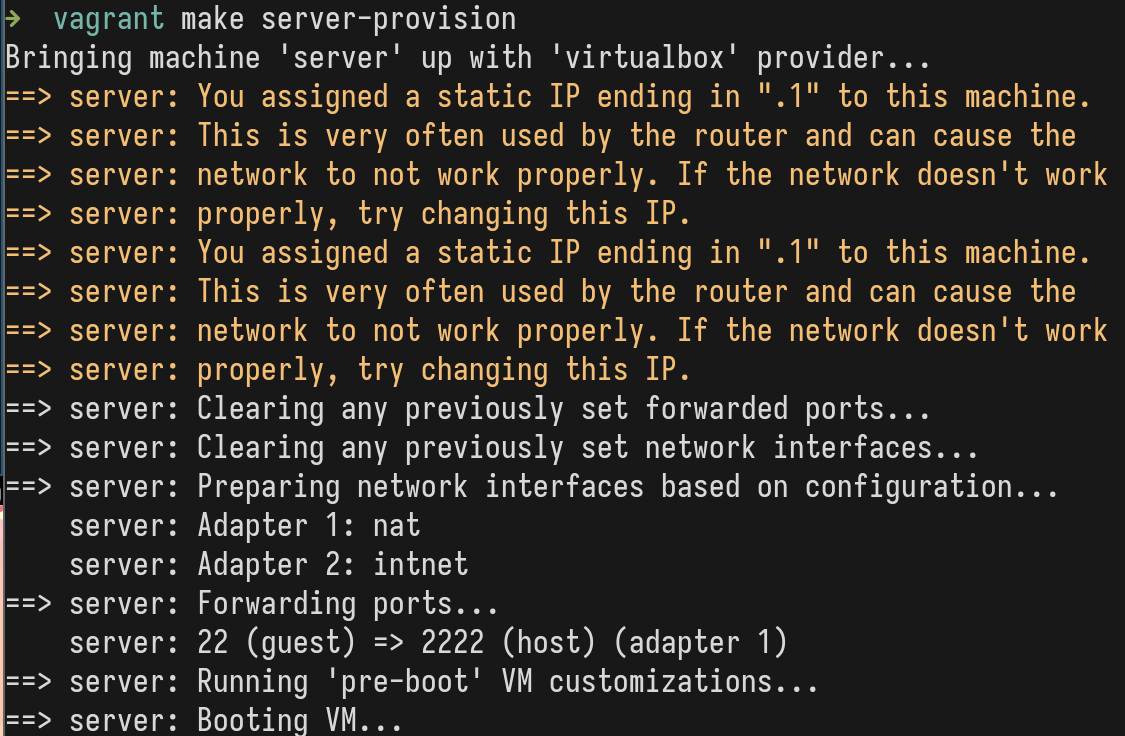
\includegraphics[width=0.7\textwidth]{../images/img11.png}
        \captionof{figure}{Фиксирование изменений настроек сервера.}
        \label{img:11}
    \end{center}
    \begin{center}
        \centering
        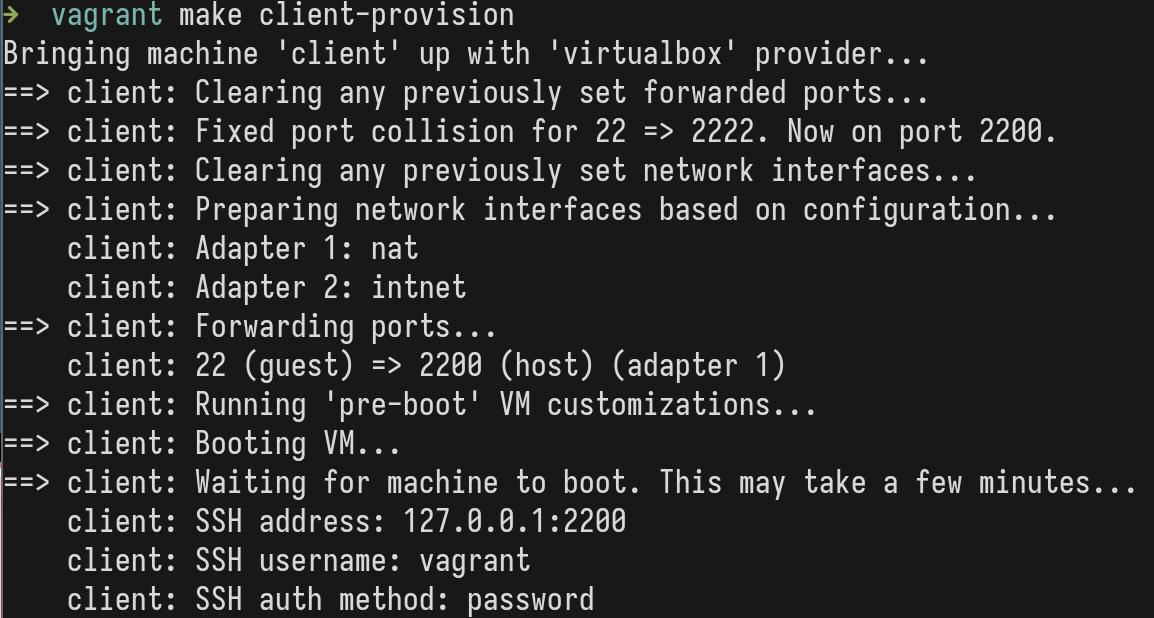
\includegraphics[width=0.7\textwidth]{../images/img12.png}
        \captionof{figure}{Фиксирование изменений настроек клиента.}
        \label{img:12}
    \end{center}

    \item Залогинились на сервере и клиенте под созданным пользователем. Убедитесь, что в терминале приглашение отображается в виде dastarikov@server.dastarikov.net на сервере и в виде dastarikov@client.dastarikov.net на клиенте (Рис. \ref{img:13} и \ref{img:14}).
    \begin{center}
        \centering
        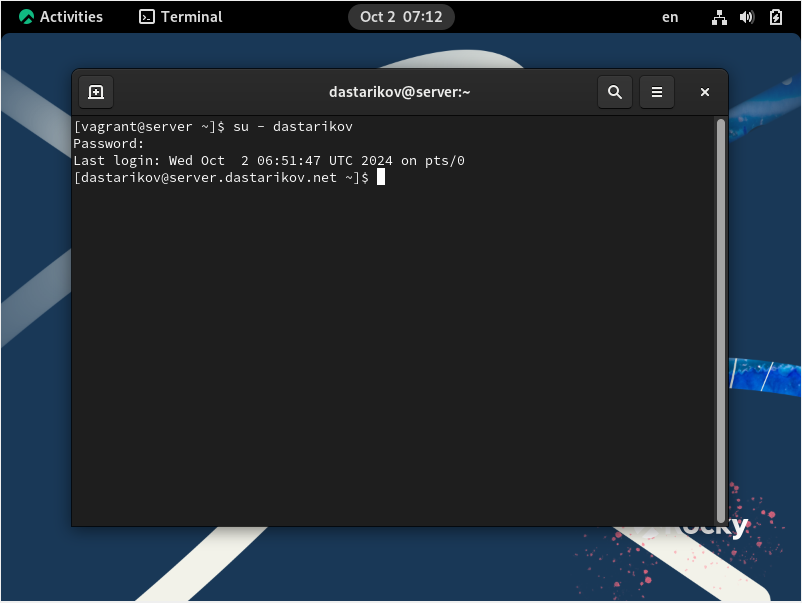
\includegraphics[width=0.7\textwidth]{../images/img13.png}
        \captionof{figure}{Проверка отображения приглашения на сервере.}
        \label{img:13}
    \end{center}
    \begin{center}
        \centering
        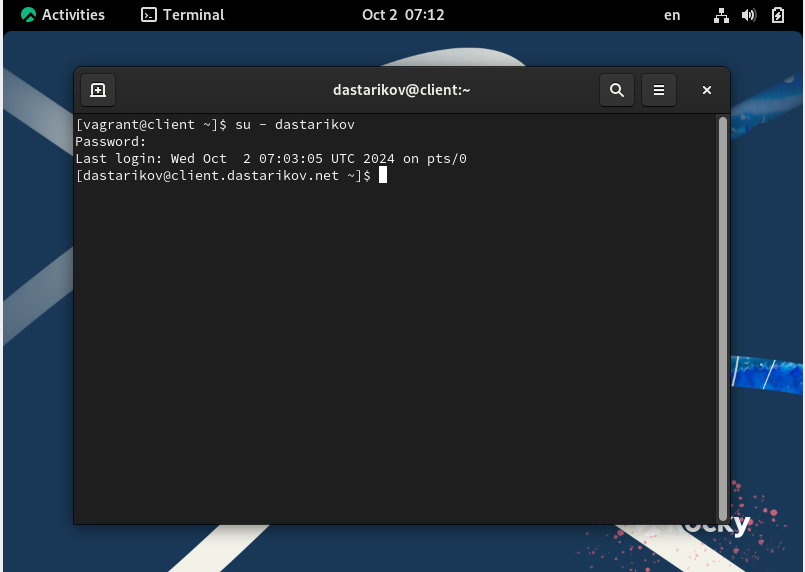
\includegraphics[width=0.7\textwidth]{../images/img14.png}
        \captionof{figure}{Проверка отображения приглашения на клиенте.}
        \label{img:14}
    \end{center}

    \item Выключили виртуальные машины.
\end{enumerate}

\subsection{Ответы на контрольные вопросы}
\begin{enumerate}
    \item Для чего предназначен Vagrant?
        Vagrant используется для создания и конфигурирования виртуальной среды разработки, при чем создаваемое окружение можно легко повторять и переносить.
    \item Что такое box-файл? В чём назначение Vagrantfile?
        Box\-файл содержит образ виртуальной машины, Vagrantfile, в котором дается описание машины и информация, как настроить и подготовить ее к работе.
    \item Приведите описание и примеры вызова основных команд Vagrant.
        \begin{itemize}
            \item Создание и запуск виртуальной машины: \texttt{vargrant up}
            \item Вход: \texttt{vagrant ssh}
            \item Остановка маишны: \texttt{vagrant halt}
            \item Удаление собранной машины: \texttt{vagrant destroy}
        \end{itemize}
    \item Дайте построчные пояснения содержания файлов vagrant-rocky.pkr.hcl, ks.cfg, Vagrantfile, Makefile
        \begin{itemize}
            \item Файл vagrant-rocky.pkr.hcl

                Блок packer устанавливает, что для работы необходимы версии vagrant и VirtualBox не ниже 1 (\texttt{version = "$\sim$> 1"}).

                Затем идут блоки variable, где задаются переменные, которые будут использоваться в работе скрипта, например имя ВМ, версия, размер дискового пространства, архитектура процессора и т. д. 

                Блок source задает конфигурацию сборщики с возможностью переиспользования. В нашем случае задаются параметры сборки виртуальной машины в VirtualBox, какой образ использовать, сколько выделить оперативной памяти, ядер процессора.

                Последний блок build описывает сам процесс сборки. Здесь указаны скрипты, которые будут запущены: настройка каталогов, установка необходимых для работы утилит.

            \item ks.cfg

                В этом файле мы задаем настройки для установки дистрибутива, которые обычно выбираются пользователем вручную при установки дистрибутива. Определяем системный язык, необходимые раскладки клавиатуры (русская и английская), логин и пароль root-пользователя, настраиваем swap.
            \item Vagrantfile

                Описываем конфигурацию запуска виртуальных машин сервера и клиента: количество оперативной памяти, видеопамяти, имя хоста, настройки VBoxAddtions.
            \item Makefile

                Содержат скрипты для программы make, упрощающие работу с vagrant. Содержит следющие цели: addbox, client-destroy,client-halt, client-provision, client-up, plugins, server-destroy, server-halt, server-provision, server-up, каждая из которых вызавает утилиту vagrant с соответствующими параметрами.
        \end{itemize}

\end{enumerate}
\newpage
\section{Выводы}
В рамках лабораторной работы познакомились с интструментом Vagrant и подготовили лабораторный стенд.
\end{document}
